
\chapter{Methods}
\label{ch:Methods}
This chapter covers the procedures involved in this research, from data collection to the proposed DL model's architecture and its training, how it is evaluated, and all the tools used during this study. It provides an explanation of how the solution for this study works and its justification.

%----------------------
\section{Data Collection}
\label{sec:DataCollection}
%----------------------
The dataset for this study consists of fluid flows interacting with an obstacle. Its purpose is to train and test the neural network solution proposed in this research. The fluid flows are generated using a numerical method, as is typically done in computational fluid dynamics simulations. The sequences represent the evolution of the fluid flow in space and time; therefore, this dataset could be considered two-dimensional Time Series data (See Section~\ref{sec:TimeSeries}).

Each fluid flow is a sequence of $400$ frames representing the state at a given time. The frames are a two-dimensional grid discretization of the simulated space, with a resolution of 200-width by 100-height cells. The values in the cells represent either the fluid's velocity at the position or -1 if it belongs to the obstacle. 

All the fluid flows in the dataset have a Reynolds number of 220 and flow from left to right, interacting with an obstacle with several dimensions and positions. These obstacles are either circumferences or ellipses, as shown in Figure~\ref{fig:cfd_obstacles}. Circumferences are simple shapes to model and are usually used to demonstrate fluid flow simulations. In contrast, ellipses are an easy simplification of an aircraft wing cross-section with different dimensions and inclinations (known as the ``angle of attack").

\begin{figure}[!h]
    \centering
    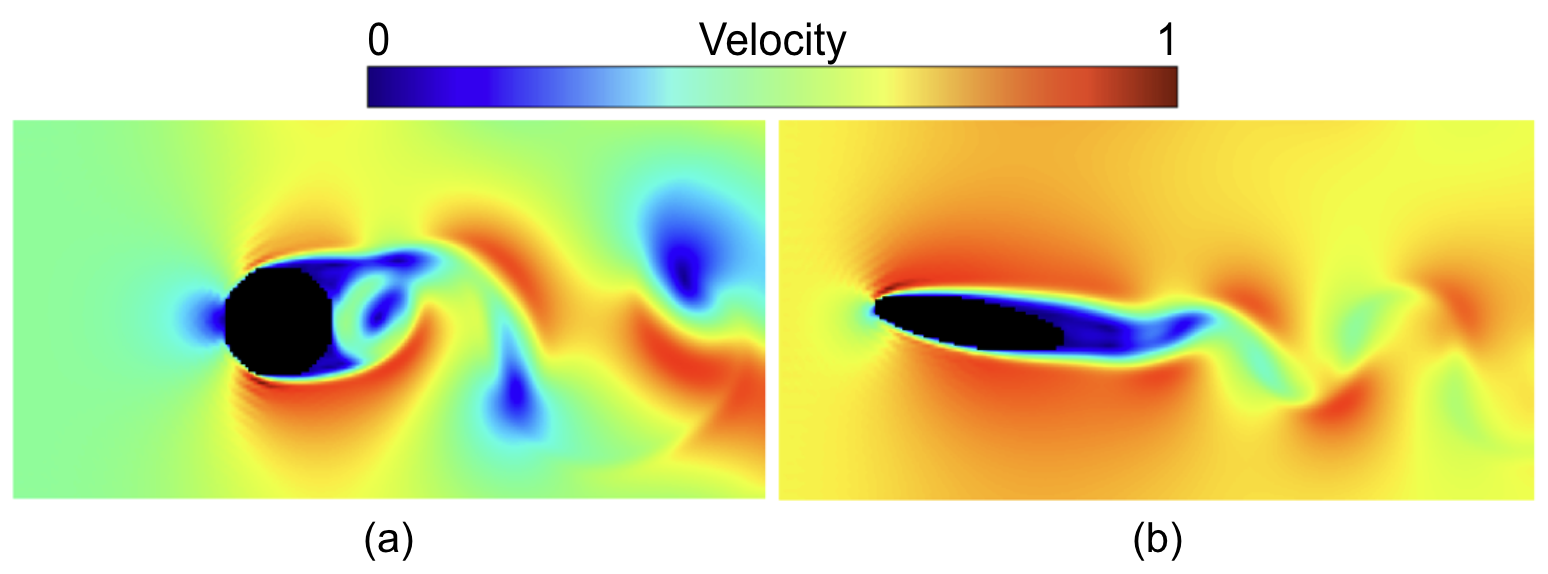
\includegraphics[width=0.9\linewidth]{images/cfd_obstacle_examples.png}
    \caption{Two CFD frames from different sequences showing the (a)circumference and the (b)ellipse obstacles}
    \label{fig:cfd_obstacles}
\end{figure}

In aeronautics, several pre-defined airfoils shapes (NACA airfoils) have been studied for the design of aircraft wings \cite{abbott_ira_h_summary_1945}; in particular, the NACA 2412 is used in the popular Cessna 172 Skyhawk. Figure~\ref{fig:naca_airfoils} shows examples of those airfoils. However, these shapes are very complex to calculate. As an alternative for this work, an ellipse shape was chosen as an approximation to the NACA airfoils. The ellipse geometry has a smooth, curved shape that can resemble the streamlined profile of the airfoil. It can provide a good approximation for the leading and trailing edges, capturing the essential aerodynamic characteristics while simplifying the complex geometry of the airfoil. This approximation is particularly useful for preliminary design and analysis, where exact precision is less critical. It allows for easier mathematical manipulation and analysis compared to the exact airfoil shape.

\begin{figure}[!ht]
    \centering
    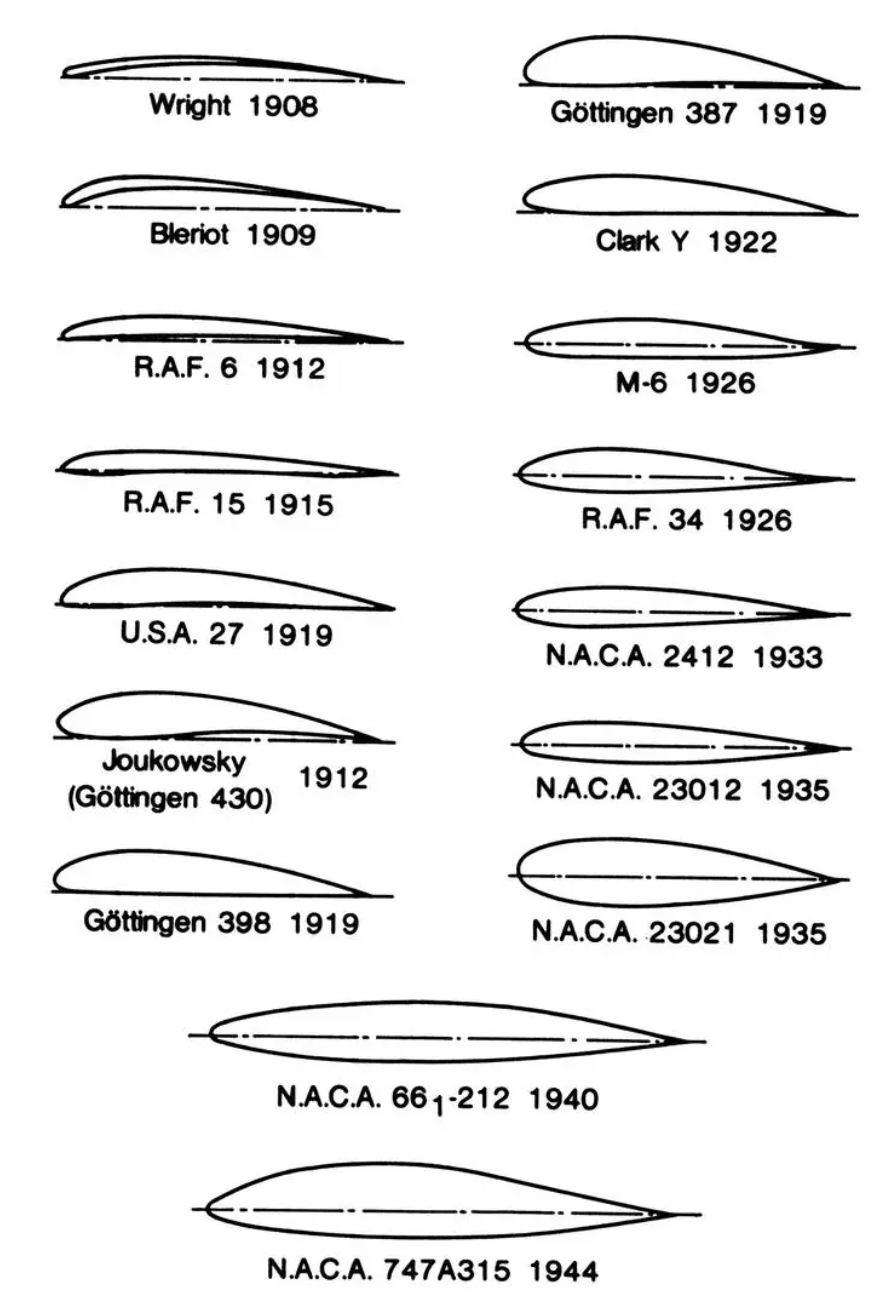
\includegraphics[width=0.6\linewidth]{images/naca_airfoils.png}
    \caption{The historical evolution of airfoil sections from 1908-1944. Credit: NACA-NASA}
    \label{fig:naca_airfoils}
\end{figure}

\subsection{Definitions}
The fluid flow sequence data can be represented in the following mathematical way. Data is taken from velocity observations in a spatial region on a $W \times H$ grid, which consists of $W$ columns and $H$ rows. Each grid cell has a velocity measurement that varies over time $T$.

\begin{defn}
    \label{defn:T}
    Let $T$ be a finite period of time and $t_i \in T$, where $i \in \{0,1,..., T\}$, is a time instance.
\end{defn}

We can then mathematically represent a fluid flow sequence as follows:

\begin{defn}
    \label{defn:fluid_flow_sequence}
    A fluid flow sequence is represented by a tensor $X \in \mathbb{R}^{T \times W \times H}$, where $x\in X$ and $x \in \mathbb{R}^{W \times H}$ is a velocity observation or fluid state at any given time $t \in T$.
\end{defn}

\begin{defn}
    \label{defn:window}
    Let $\mathcal{W}$ be a window of time $\subseteq T$, where $\mathcal{W}$ is of size $m$ and $1 < m < T$.
\end{defn}

When observations of $x \in X$ are recorded periodically over a time period $T$, we can think of them as a sequence of frames $x_0, x_1, x_2, ..., x_i, ..., x_T$. For this research, the spatiotemporal sequence generation problem is to generate the next most likely frame $x_i$ observation, given a window of previous observations $x_{i-m}, ..., x_{i-2}, x_{i-1}$. The problem can be formalized by equation~\ref{eq:generation-problem}, where $g$ represents the \textit{generate} function performed by the model.

\begin{equation}
    x_i = g(x_{i-m}, ..., x_{i-2}, x_{i-1}) 
    \label{eq:generation-problem}
\end{equation}

% -------------------------------------------------------
\section{Data Preparation}
\label{sec:DataPreparation}
% %-------------------------------------------------------
Before the data is used to train and evaluate the model, the following preprocessing steps are applied to transform the data: 1) data normalization, 2) data slicing, and 3) dividing the dataset into a training and testing set.

\begin{enumerate}
    \item \textbf{Data normalization:} First, the data is normalized by scaling the velocity values between 0 and 1. This data normalization improves the gradient descent optimization during the neural network's training, which is a common requirement for deep learning methods. This scaling is done according to Equation~\ref{eq:min-maxscaling} below.

        \begin{equation}
            v_{scaled} = \frac{v-v_{min}}{v_{max} - v_{min}}
            \label{eq:min-maxscaling}
        \end{equation}
    
    This scaling technique provides robustness to very small standard deviations in the dataset's velocity values. During this process, the obstacle cells are left with a value of -1 to distinguish them from the fluid while maintaining the velocity values in the 0 to 1 range.
    
    \item \textbf{Data slicing:} This step focuses on creating simulated sub-sequences to train the model. The input and output datasets are generated using the original dataset, which consists of the simulated [fluid] sequences. The model takes as input a specific window $\mathcal{W}$ consisting of $m$ frames from the simulated sequence of size $T$; it then uses this window to generate the next frame. Since $m<T$, the length of the input dataset elements must be reduced to match the this window. To do this, each original sequence is segmented into sub-sequences of length $m$ (size of $\mathcal{W}$). After segmenting the original sequence of size $T$, it results in more than one sub-sequence of size $m$ in the input dataset.
    
    Figure~\ref{fig:data_slicing} illustrates this process, where the input dataset to the model (the set of fluid sub-sequences $X$ of size $m$ over a time window $\mathcal{W}$ using definition~\ref{defn:window}), will be used to generate the output set (the next set of frames). During the training step, the model will learn how to infer $x_t$ from the previous $m$ frames (see  Equation~\ref{eq:generation-problem}).
 
    \begin{figure}[H]
        \centering
        % 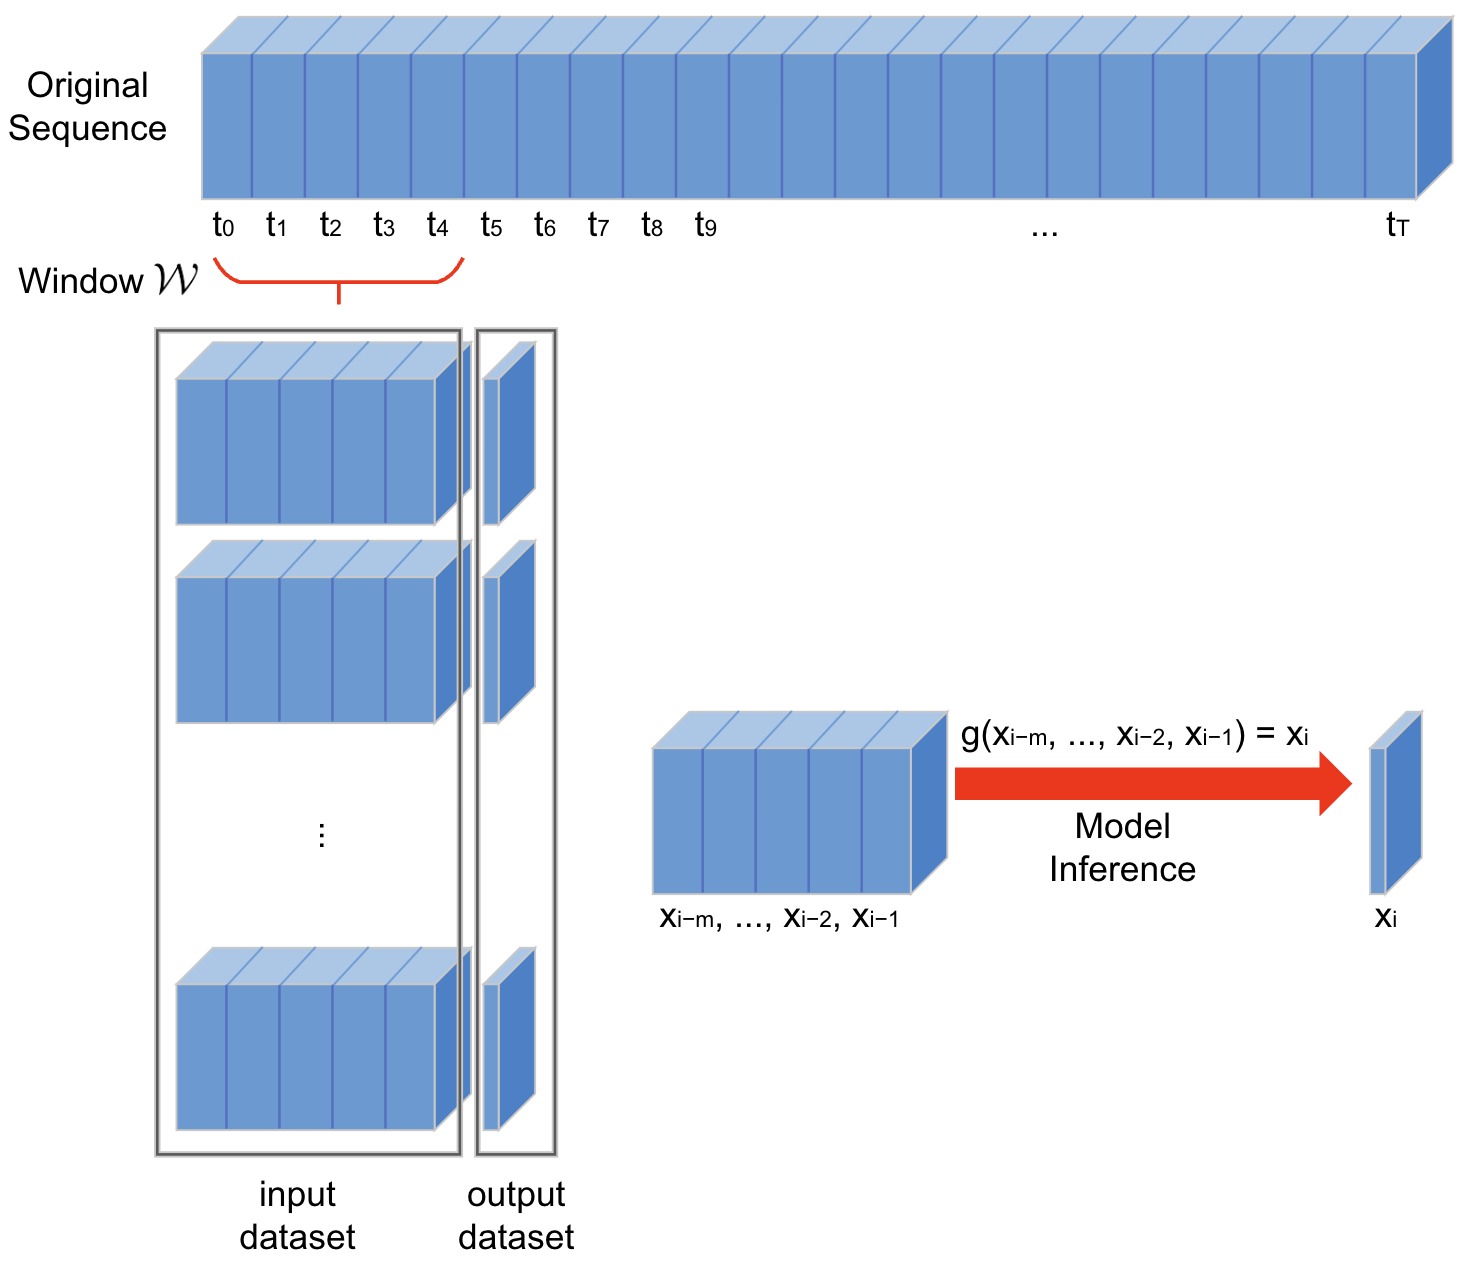
\includegraphics[width=0.9\linewidth]{images/data_slicing.png}
        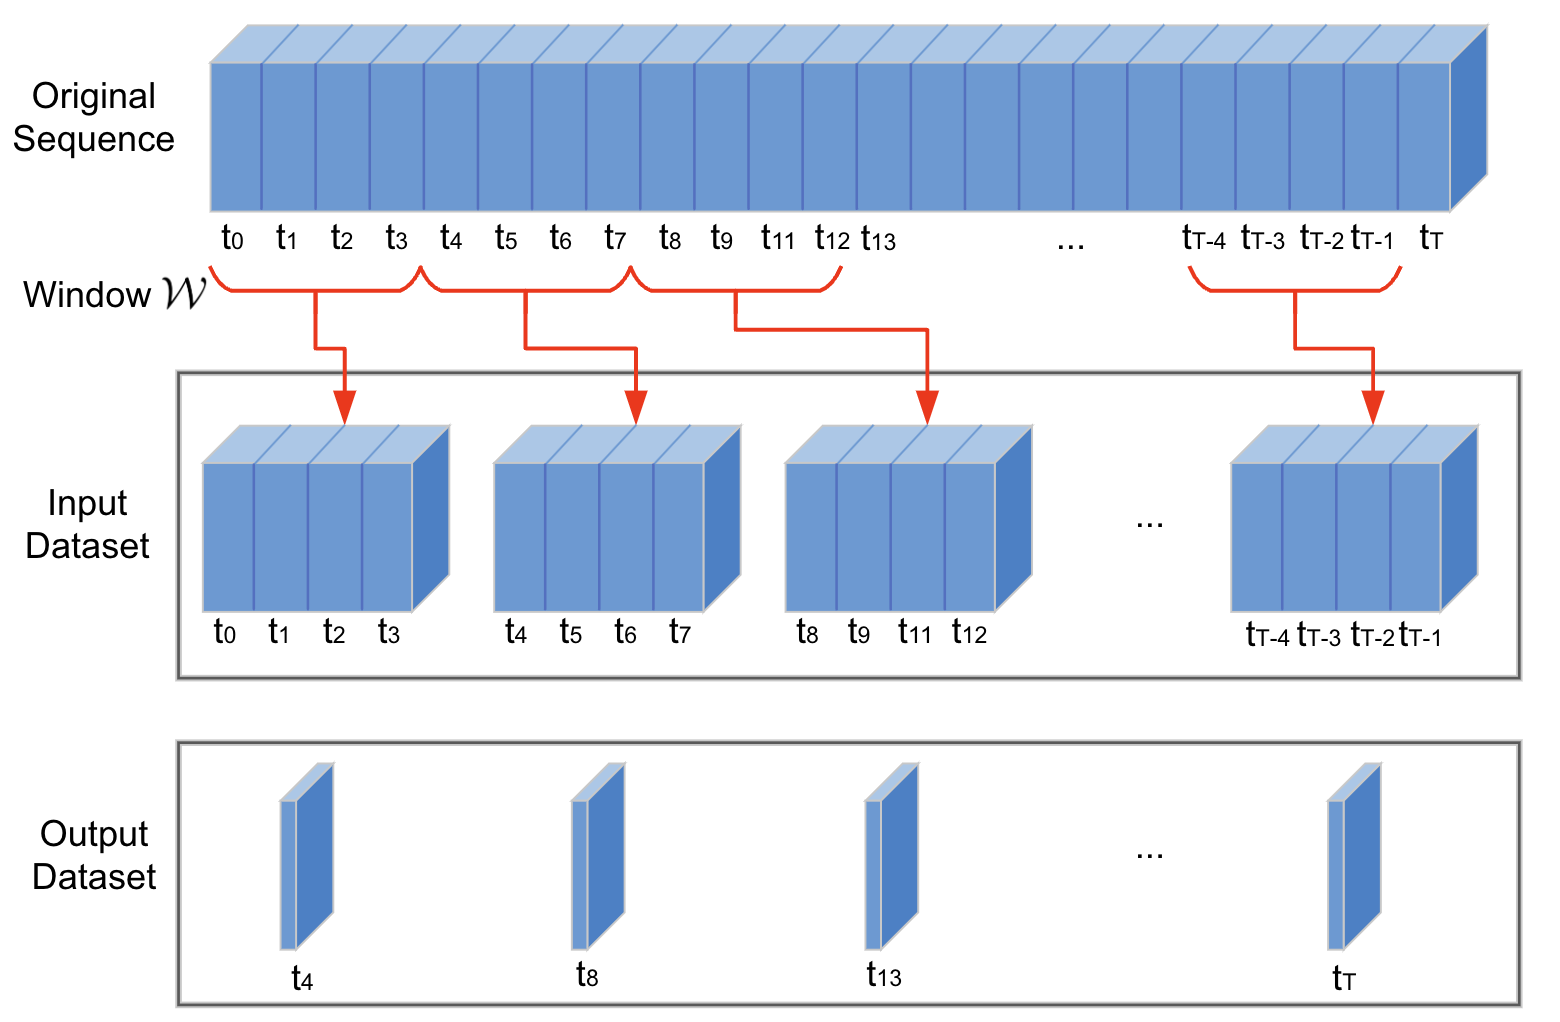
\includegraphics[width=0.9\linewidth]{images/data_slicing_v2.png}
        \caption{Slicing of sequence into $\mathcal{W}$ sub-sequences used to train the model.}
        \label{fig:data_slicing}
    \end{figure}

    \item \textbf{Training, Validation, and Testing sets:} Finally, the dataset is shuffled and then randomly divided into training, validation, and testing sets with an 8:1:1 ratio, respectively. This is done to validate and test the model using the cross-validation method with samples not used during training. This aims to provide an unbiased evaluation of the model's efficacy, which -- ideally --  should appropriately generalize (for new data) without over-fitting (training data). 
    
\end{enumerate}


%----------------------
\section{Model Architecture}
\label{sec:ModelArchitecture}
%----------------------
The DL solution proposed in this research is an end-to-end model, meaning it will perform all the tasks from data input to generating the fluid flow simulation output in one unified process. In contrast, other related research uses machine-learning or DL techniques for only a specific part of the simulation, leaving the rest to a classical numerical method and making the process more complex. A benefit of our simple approach with only one task is eliminating the need for complex pipelines between separate parts in the simulation process, thus reducing development time and potential sources of error. Additionally, end-to-end models can better adapt to diverse datasets and changing environments since they learn directly from raw data, capturing intricate patterns and relationships that might be missed in traditional approaches, like DNS.

The goal of this model is to generate predictions of a fluid flow's evolution. To accomplish this, the model looks at past states in the flow and generates the following future state. The future state can then be used as an input to continue generating new states in the simulation. This step can be repeated as many times as necessary as a feedback loop shown in Figure~\ref{fig:feedback_loop} below. As a result of this feedback loop, the model can produce a long fluid flow sequence. In Figure~\ref{fig:feedback_loop}.a we can see how the resulting frame is put at the end of the input sequence to generate a new frame (see Section~\ref{subsec:Generator}). Figure~\ref{fig:feedback_loop}.b shows how the model looks at a certain window of the frame and moves forward in time to generate the rest of the sequence. At the beginning of a simulation, the model uses an initial condition or ``ground truth" represented by a number of frames equal to the sliding window ($\mathcal{W}$). As $\mathcal{W}$ slides, new frames are generated, which are in turn used to generate more subsequent frames. Eventually, an entire sequence can be generated, knowing only the first frames from the initial fluid's condition, and the rest are completely generated by the model.

\begin{figure}[!htbp]
    \centering
    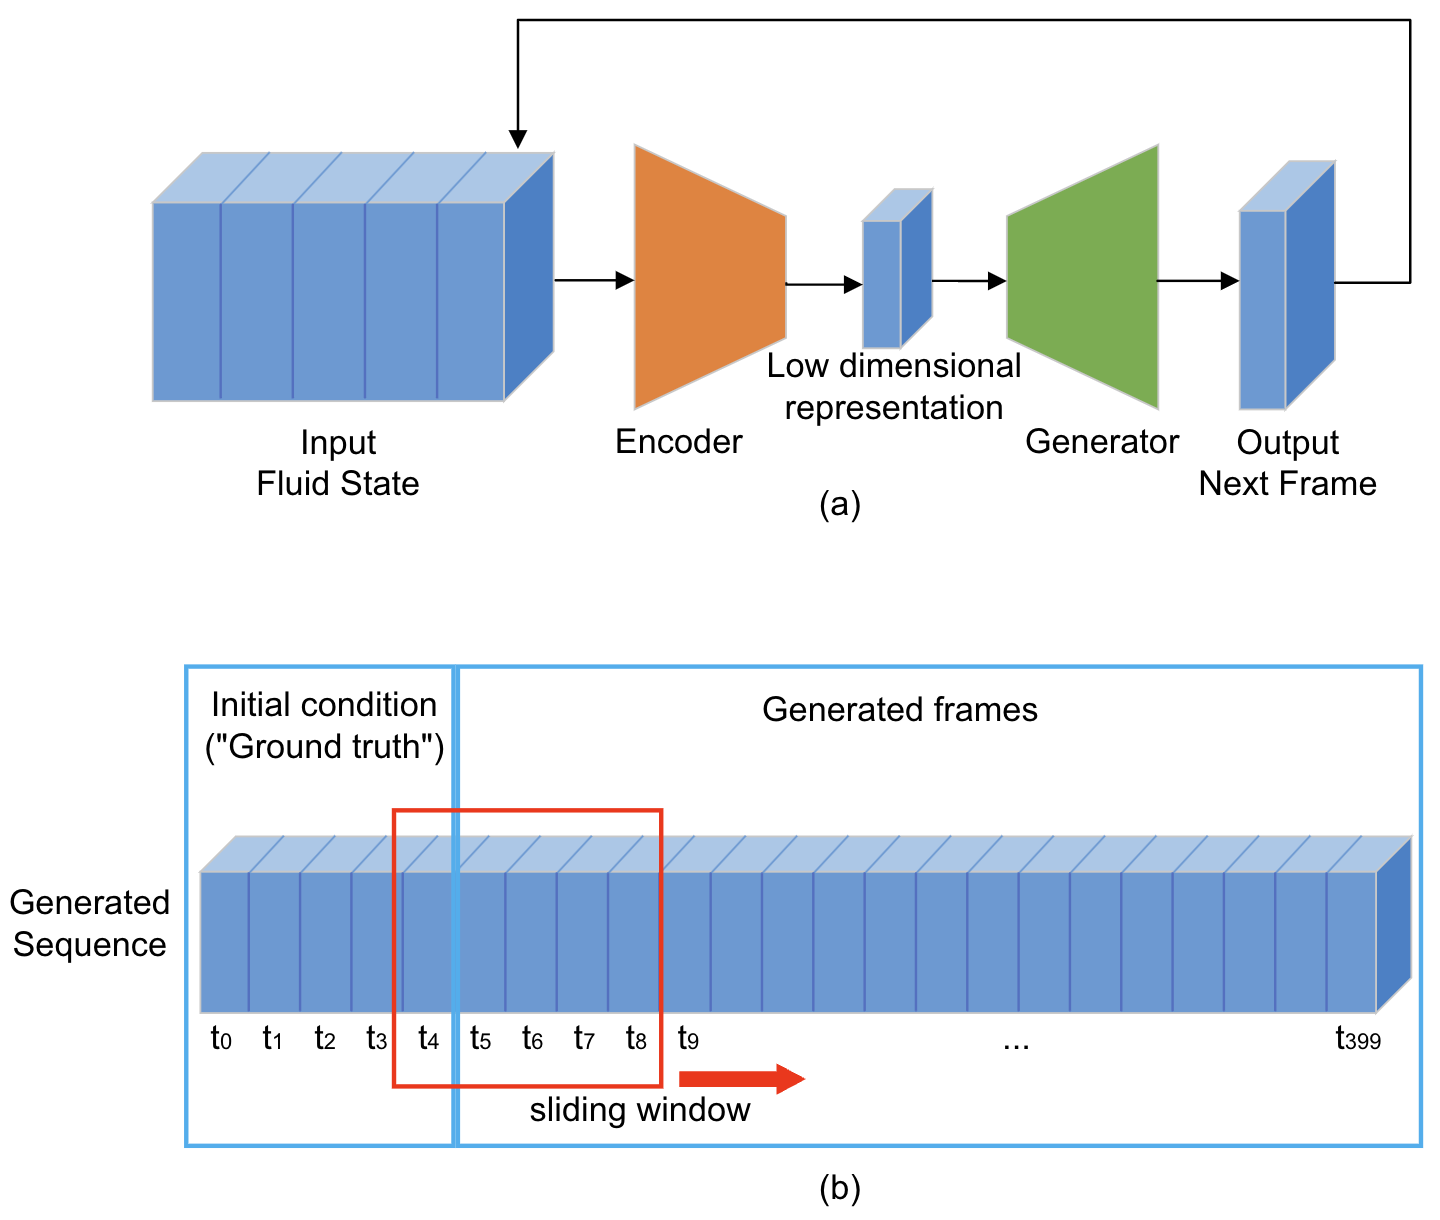
\includegraphics[width=1\linewidth]{images/feedback_loop.png}
    \caption{Diagram showing a) the flow between the model's main components and b) sliding window approach for prediction.}
    \label{fig:feedback_loop}
\end{figure}

Because of the data's spatiotemporal characteristics, the neural network has to be capable of analyzing and learning the evolution of fluid flows in two dimensions: space and time. A CNN (See Section~\ref{sec:CNN}) can help understand the spatial structure of the fluid to extract the flow's features and patterns in space. Additionally, the model needs to ``remember" what happened in the past to produce the next state, so it needs a memory mechanism that can be provided by a recurrent neural network such as an LSTM (See Section~\ref{sec:LSTM}), commonly used in Natural Language Processing tasks. As mentioned before, these two types of neural networks have been combined to create the ConvLSTM (See Section~\ref{sec:ConvLSTM}) as an extension of the LSTM network that can also ``look" for features in space and time. For this reason, the ConvLSTM network was chosen to implement the neural network architecture proposed in this study.

Because this data has many dimensions and complexities, a dimensionality reduction is applied to capture the principal components of the flow before generating the next frame. This ensures that the model will rely on a minimal representation of the fluid flow that accurately describes its behavior. For this model architecture, the dimensionality reduction is implemented by an Autoencoder (See Section~\ref{sec:Autoencoders}) neural network that can produce it as part of the same model.

\begin{figure}[!htbp]
    \centering
    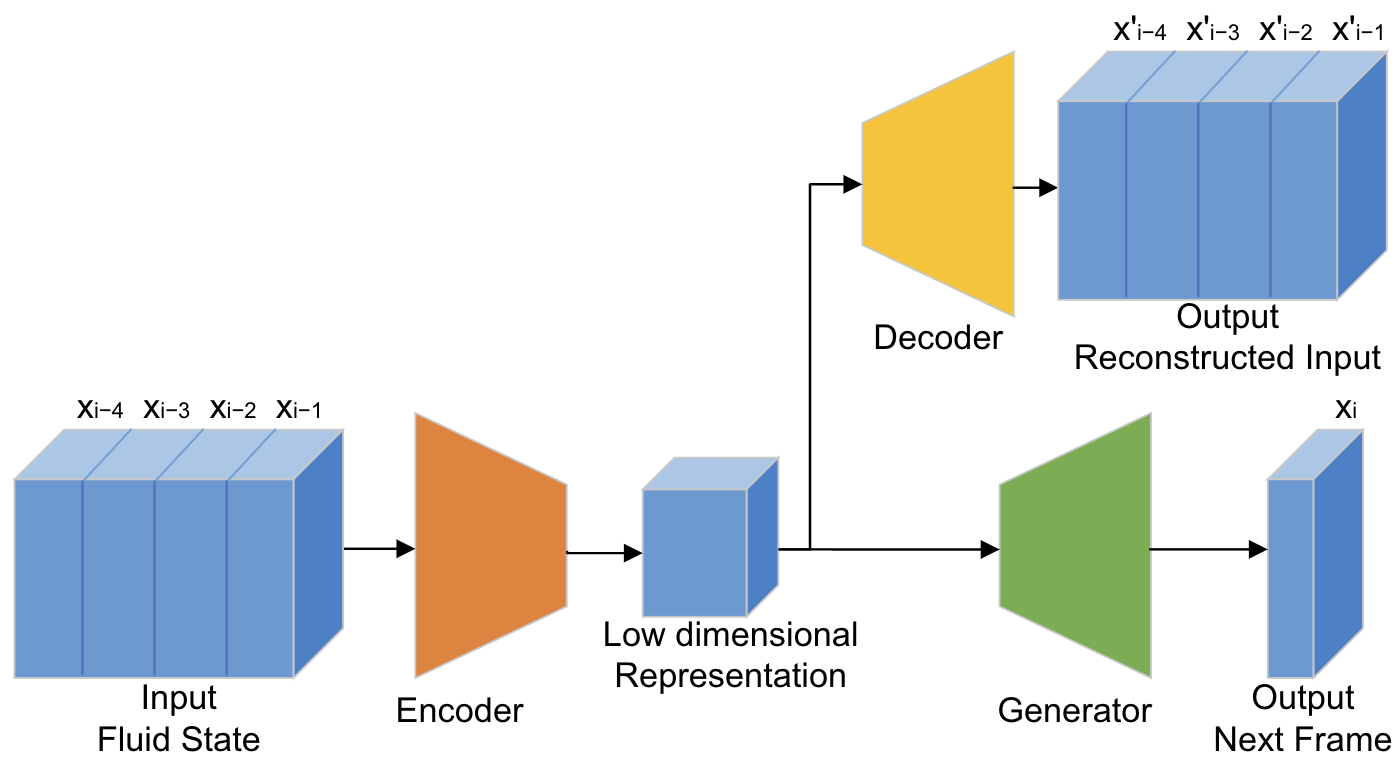
\includegraphics[width=0.8\linewidth]{images/model_schematic.png}
    \caption{Schematic diagram of the model architecture}
    \label{fig:model_schematic}
\end{figure}

In summary, the model has two main parts, as shown in Figure~\ref{fig:model_schematic}: 1) an Encoder that reduces the data's dimensionality and 2) a Generator that gets a representation of the past frames and creates the next one.

\subsection{Encoder}
\label{subsec:Encoder}
The Autoencoder is a neural network architecture composed of an Encoder and a Decoder, and it is used for dimensionality reduction (See section~\ref{sec:Autoencoders}). It takes data with many dimensions and creates a representation of this data in a lower-dimensional space. It is used similarly to classical statistical methods, such as singular value decomposition or principal component analysis. As explained in the related works chapter~\ref{ch:RelatedWork}, autoencoders were previously used for fluid flow analysis, such as identifying the main components in a fluid flow and identifying eddies in the flows. It has also been used for dimensionality reduction for other methods that are not deep learning models. 


\subsection{Generator}
\label{subsec:Generator}
The generator takes the lower-dimensional representation of the fluid flow state and generates a new frame in the sequence. Using a lower representation of the data instead of all the original dimensions makes this work easier because the generator will get as input the main components that can describe the flow. 


%----------------------
\section{Model training}
\label{sec:ModelTraining}
%----------------------
The Encoder is trained in conjunction with the Decoder component, which takes the lower dimensionality representation and tries to reconstruct the original input. If the decoder can reconstruct the original data using the reduced representation from the encoder, this means that the representation captures the main elements of the sequence, and the encoder works correctly. This decoder is auxiliary and discarded once the model’s training is completed.

Cross-validation \cite{bengio_practical_2012} is used to ensure that the model performance generalizes well to unseen data during training. This method, commonly used in machine learning, involves splitting the dataset into three parts: a training set, a validation set, and a testing set. The training set is used to train the model, and simultaneously, the validation set is used to evaluate the model's performance during training. Once the model is trained and optimized, it is tested on a separate and unseen test dataset to assess its generalization performance. This technique also helps prevent overfitting by providing an independent dataset for model evaluation. It ensures that the model's performance estimates are more reliable and indicate its performance on new data.

The neural network training job was distributed across the two GPUs available on the server. This was done using the Mirrored Strategy, a synchronous data parallelism algorithm for neural network training. This algorithm replicates the model on both GPUs and splits the dataset between devices. The CPU prepares and sends the data batches to the GPUs. During training, each GPU performs a forward pass over the model on different input data to compute the loss function; subsequently, gradients are calculated on each device based on that loss. Both sets of gradients are then combined with an all-reduce operation by averaging them and re-distributing them across devices to update the model parameters on each replica, synchronizing them. This process is repeated for each data batch for every training epoch.


%----------------------
\section{Hyperparameter Optimization}
\label{sec:HyperparameterOptimization}
%----------------------
The model architecture and training have specific characteristics or hyperparameters that can take various possible values. These hyperparameters impact the model's performance, i.e., different combinations of such values may result in different model efficacy; consequently, it is important to find a suitable hyperparameter combination to optimize the model efficacy.

Hyperparameter optimization with Random Grid Search \cite{bengio_practical_2012} in ML involves systematically exploring a predefined hyperparameter space by randomly sampling combinations of hyperparameters, rather than exhaustively searching through all possible such combinations. This approach helps efficiently find an optimal set of hyperparameters for the model by balancing computational resources and exploring the parameter space. Random grid search randomly selects hyperparameter values from specified distributions and evaluates each combination using cross-validation to determine the set that yields the best performance metric. This technique can effectively search a large hyperparameter space, improving model performance without exhaustive computational costs.

The hyperparameters considered for this model are:

\begin{itemize}
    \item Learning rate: it determines the update step size of the weight in the neural network at each iteration during the optimization process, i.e., the loss function moving towards a minimum. A high learning rate can lead to rapid convergence at the risk of overshooting the optimal solution, causing the model to diverge. On the other hand, a low learning rate ensures steady convergence at the sake of a slower training process which can get stuck in local minima. This parameter significantly impacts the efficiency and effectiveness of the model training. The best training results were achieved with a learning rate of 0.001.
    
    \item Number of layers: the number of neural network layers affects the \textit{capacity} of the model to learn complex representations. In the context of this research, more layers can enable the model to capture more hierarchical features and intricate patterns in the fluid-flows. This can improve the model's performance. However, having more layers makes the model more complex and more susceptible to overfitting the training data. The model achieved the best results using 3 ConvLSTM layers on each Encoder and Decoder component and 4 ConvLSTM layers in the Generator component.
    
    \item Number of filters or kernels on each layer: convolutional filters detect spatial features in the input data. These filters enable the model to capture both spatial and temporal dependencies in the fluid flow. The number of filters impacts the model's ability to extract relevant features. Having more filters can capture more complex data patterns but at the cost of increasing computational cost. This parameter affects the accuracy and efficiency of the model. In the ConvLSTM layers of the Autoencoder, this model architecture got the best results using 64 filters in the first and last layers and 32 in the other ones. In the Generator component, the first layer uses 32 filters and 64 in the rest.
    
    \item Size of the filter: this refers to the convolutional filters' dimension to capture features of the input data. The filter size determines the scope of the local spatial region examined by the model. Larger filters can capture broader spatial patterns but may miss fine-grained details, while smaller filters focus on more localized features, potentially overlooking broader context. This impacts the model's ability to detect relevant features. The following filter sizes in the ConvLSTM layers of the architecture were used to get the best results, in order from the first to last layer of each component: the Encoder has filter sizes of 4 by 4, 3 by 3, and 2 by 2; the Decoder has filters of 2 by 2, 3 by 3, and 4 by 4; and the Generator filter sizes are 3 by 3 for all of its layers. 
\end{itemize}

In order to define a search space of hyperparameter combinations, a range of values is set for each of these hyperparameters.  Potential combinations are selected by random sampling, then a model is trained using those combinations, and the one with the best performance is selected. Once the best combination is found, the model is trained during more epochs to get the final version of the model.

When choosing the $m$ size of the window $\mathcal{W}$, several aspects were considered, e.g., the amount of ``historical'' data used to generate a prediction. Similar to the Exponential Moving Average (EMA) heuristic \cite{kalekar_time_2004} \cite{ugli_cognitive_2023}, which can be used in time-series forecasting scenarios and LSTM models to weight the amount and relevance of historic measurements vs. predicted ones. In our case, we can think of $m$ as the amount of historical information that the model will receive to make a future prediction. In this sense, using a small window will not give enough information to the model. On the other hand, having a bigger window size provides more information and is better for the model, but if $m$ is too big, it will need too much historical information, making the model pointless. Additionally, a bigger window expands the input dimensions, so more computations would be required to compress the data to create the lower dimensional representation. This increase in computations makes the model slower to execute and train, which given our limited computational resources, could render our model impractical. In addition, since the sequences have 400 frames each, the window size $m$ has to be a divisor of 400 to split them into sub-sequences for data preparation, as explained in \ref{sec:DataPreparation}. Overall, since a window of size 2 would be too small to provide the model with enough information, a window size of 4 was chosen since it is the smallest $m$ that allows for the even division of sub-sequences while keeping the model practical.


%----------------------
\section{Proposed Architecture Details}
\label{sec:ArchitectureDetails}
%----------------------

The final model architecture has two components: the \textbf{Autoencoder} and the \textbf{Generator}. The Autoencoder is divided into the Encoder and Decoder. The window $\mathcal{W}$ of $m=4$ frames is first input into the Decoder, which creates a low-resolution representation of the simulation. Next, this low-resolution representation is input into the Generator to create the next frame state of the fluid flow. All these components are implemented in the neural network by a set of ConvLSTM layers followed by either MaxPooling or UpSampling layers. ConvLSTM layers extract features in the data by using convolutional operators called filters or kernels. MaxPooling and UpSampling layers compress or uncompress the intermediate data outputs between ConvLSTM layers. MaxPooling downsamples the input by taking the maximum value in the kernel window along the spatial dimension. UpSampling layers resize the input by interpolating its values. Figure~\ref{fig:model_detail} shows a detailed diagram of this architecture where we can see the order of these layers. In the Encoder, successive layers of ConvLSTM and MaxPooling layers downsample the data, resulting in a representation that is half the input size. This representation is then reconstructed in the Decoder by upsampling it using UpSampling and ConvLSTM layers. Each of these layers has a different amount of filters or pool windows of different sizes, respectively. 
Figure~\ref{fig:model_detail} also shows the output dimension of each layer.

\begin{figure}[!htbp]
    \centering
    \makebox[\textwidth][c]{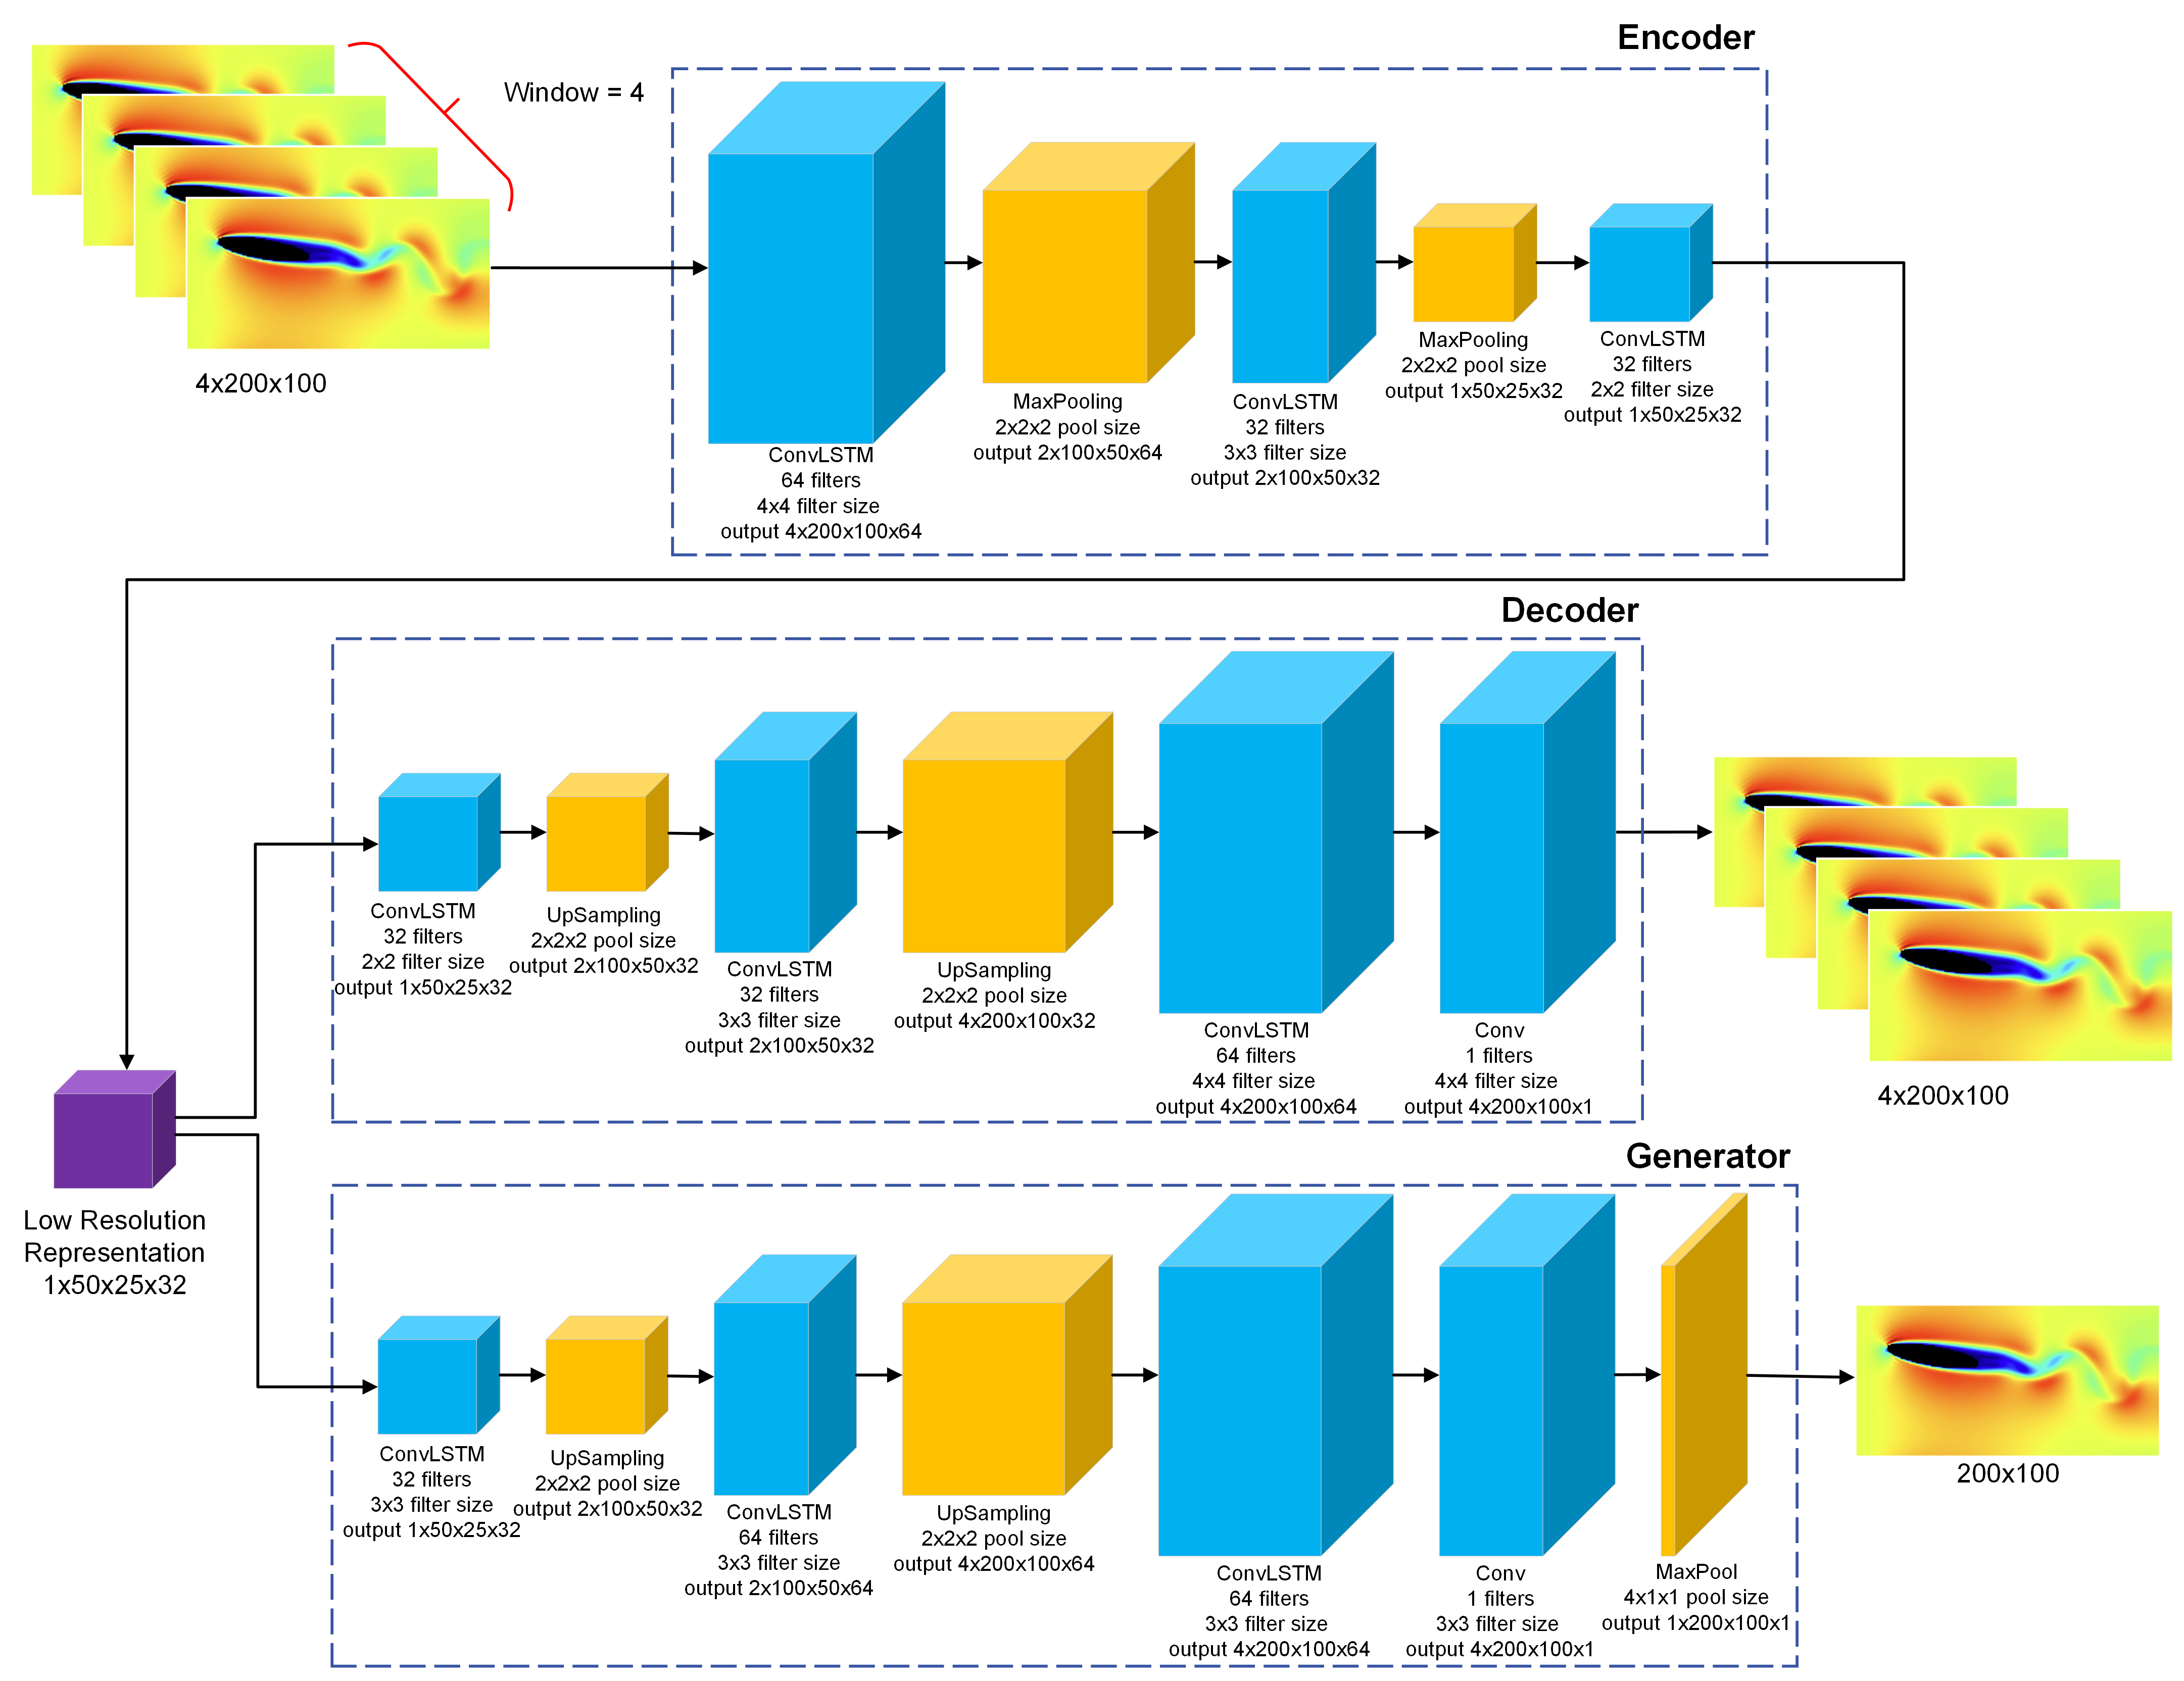
\includegraphics[width=1.3\textwidth]{images/architecture_detail.png}}
    % 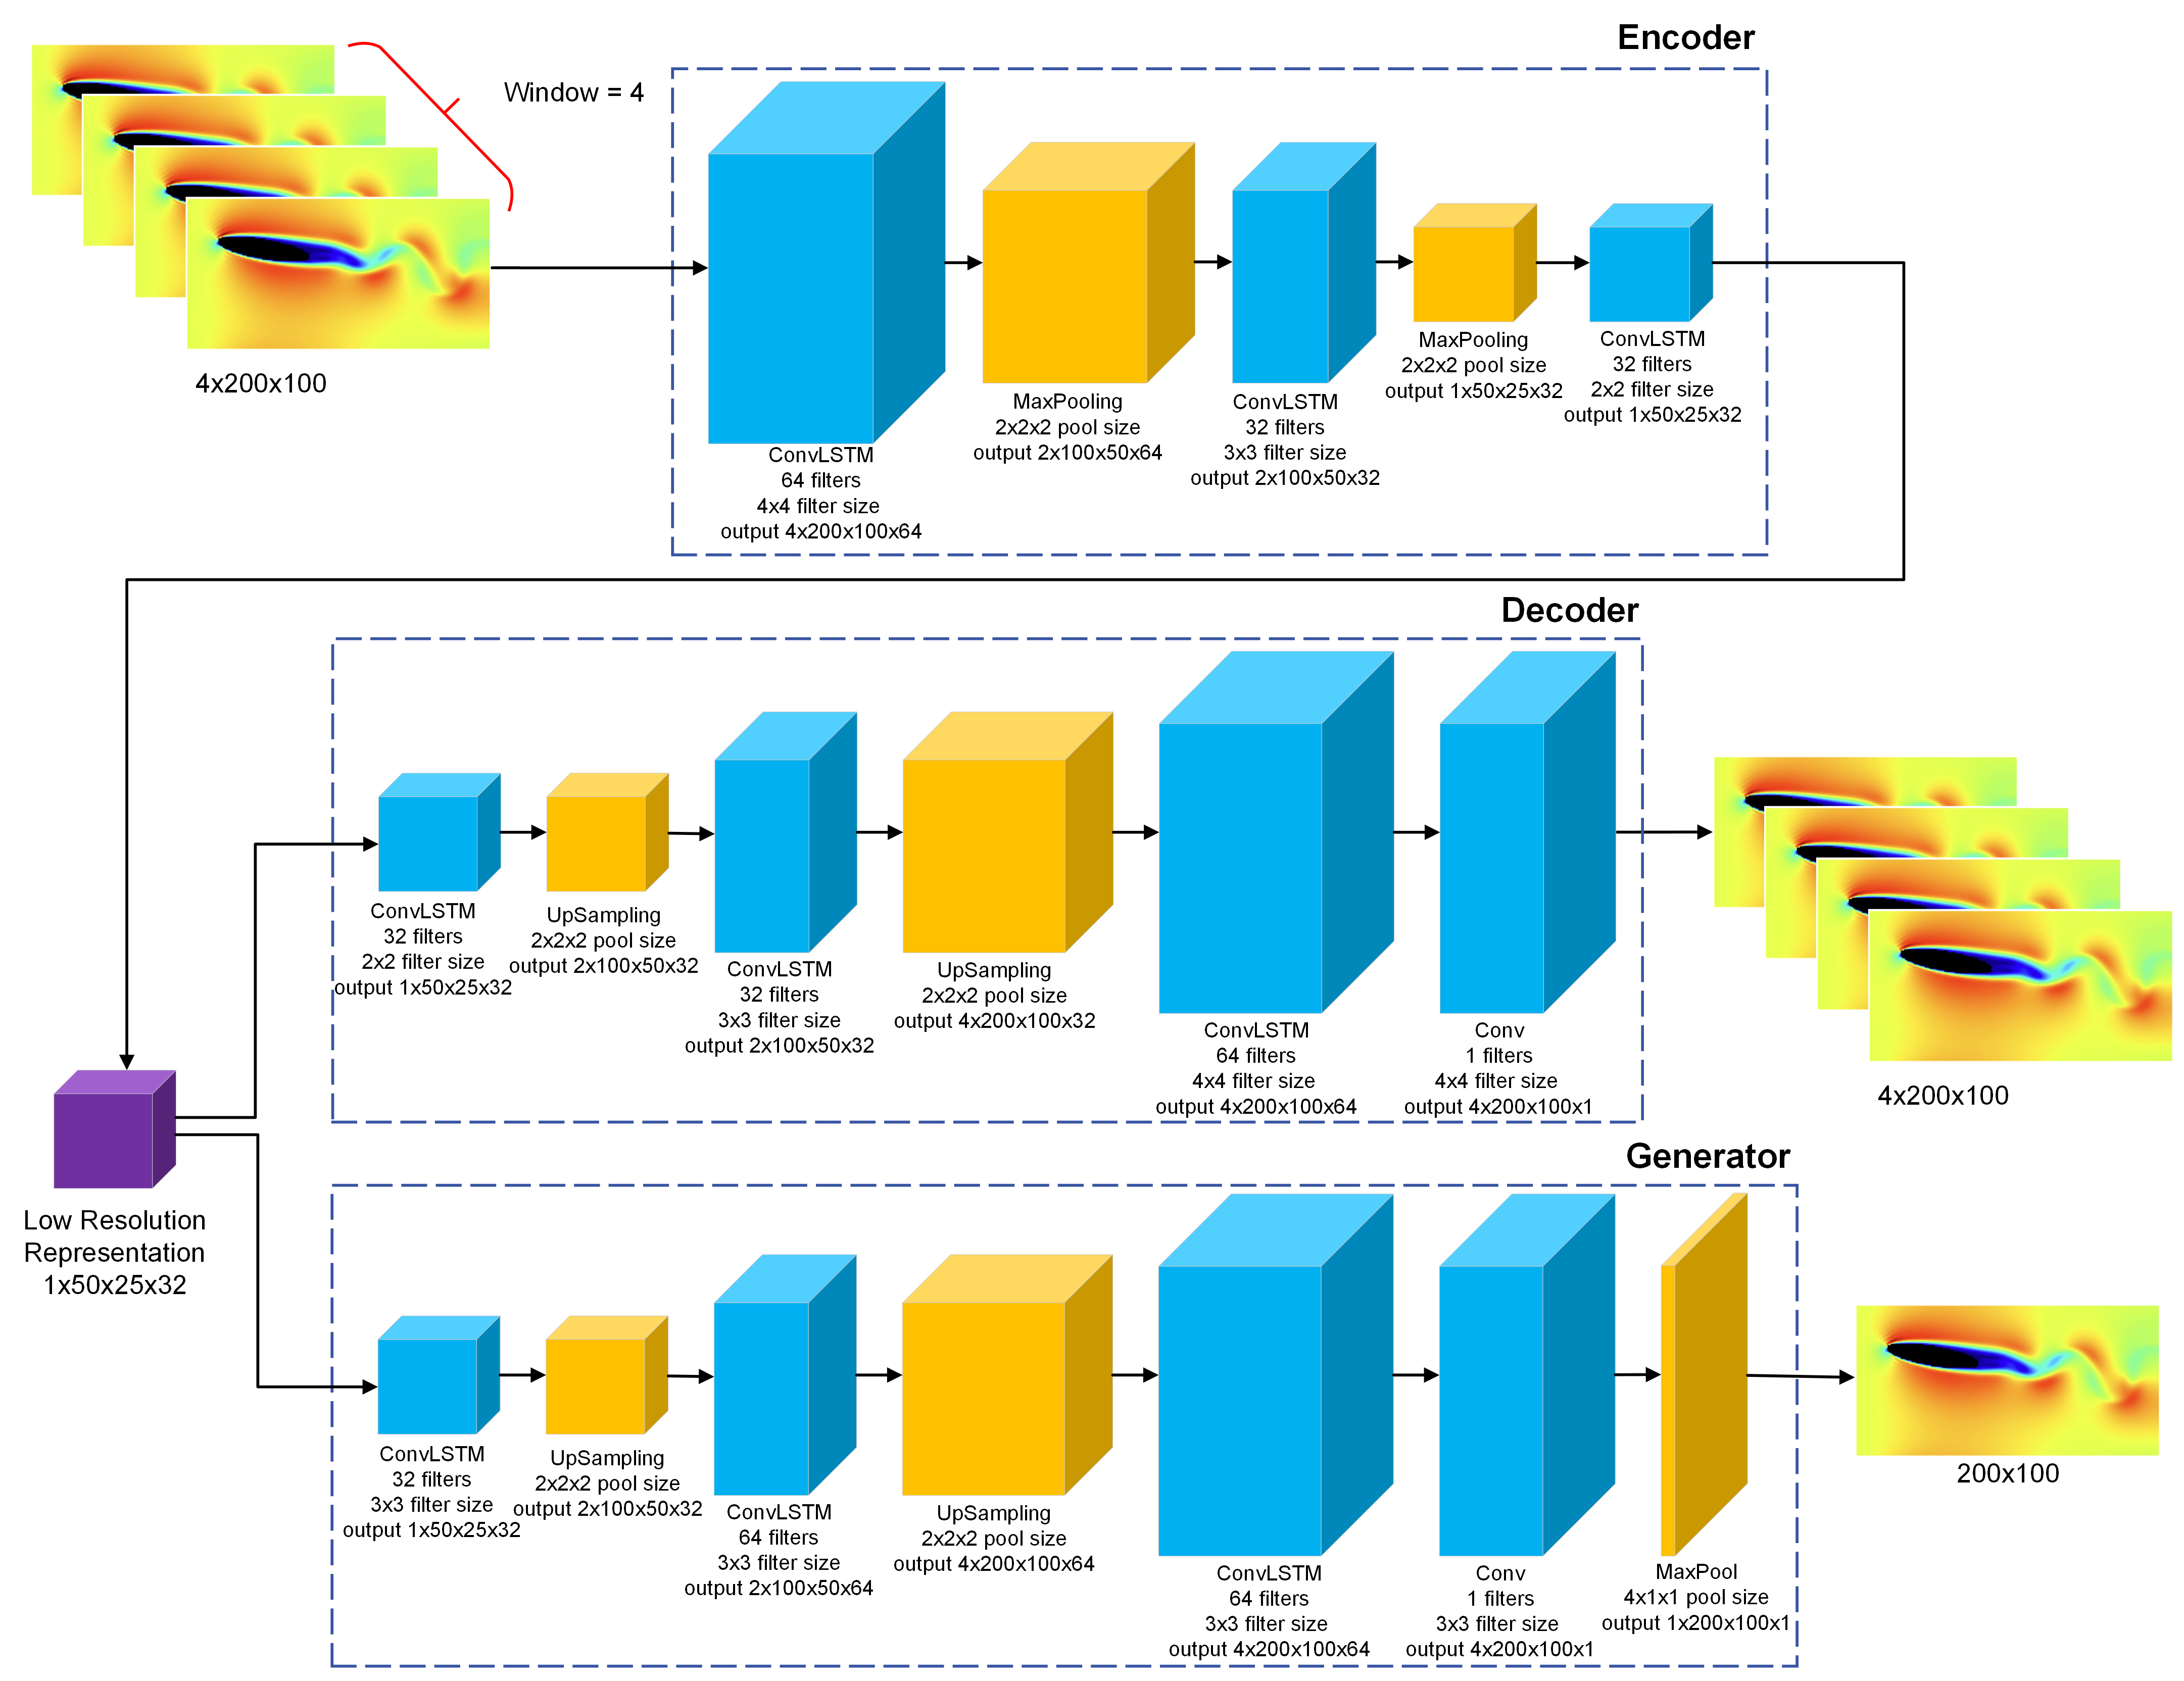
\includegraphics[width=1\linewidth]{images/architecture_detail.png}
    \caption{Detail diagram of the model architecture}
    \label{fig:model_detail}
\end{figure}

%----------------------
\section{Evaluation Methods}
\label{sec:EvaluationMethods}
%----------------------
The model evaluation is done using three strategies:
\begin{enumerate}
    \item Calculating the Mean Square Error between the original and generated simulations.
    \item Visually inspecting the simulation result by rendering an image with the generated data and comparing it with the expected data (the ground truth).
    \item Creating a histogram of frame values for the original and the generated data, these will be compared ``side-by-side" to analyze similarities and identify possible drastic differences.
\end{enumerate}

%----------------------
\section{Software and Tools}
\label{sec:SoftwareandTools}
%----------------------
For the implementation of all the methods described in the previous section, the Python \cite{python} scripting language with the following libraries: TensorFlow \cite{tensorflow} and Keras \cite{keras}, for the neural network implementations and training; Numpy \cite{numpy} and scikit-learn \cite{scikit-learn}, for data manipulation and preprocessing; and Matplotlib \cite{matplotlib}, to generate the plots and visualizations.

VS Code was used as an IDE for code implementation, and data analysis of the results was done using Jupyter Notebook \cite{jupyter}.

The server used for training and evaluation of the neural network model has the hardware specifications described in Table \ref{tab:serverHW} below.

\begin{table}[h]
    \caption{Server Hardware specifications}
    \centering
    \begin{tabular}{|c|l|}
    \hline
    \multirow{3}{*}{CPU} & Intel(R) Xeon(R) Gold 5118 CPU       \\
                         & 2.30GHz of frequency                 \\
                         & 12 cores                             \\ \hline
    RAM                  & 192 GB                               \\ \hline
    \multirow{3}{*}{GPU} & 2x Nvidia Tesla V100 with 16 GB or RAM each \\
                         & Nvidia Volta Microarchitecture       \\
                         & Compute Capability 7.0               \\ \hline
    \end{tabular}
    \label{tab:serverHW}
\end{table}

